%---------------------------------------------------------------------------------------------------------------------------------------------
%                                                            HEADER
%---------------------------------------------------------------------------------------------------------------------------------------------
% ¿Qué secciones debe contener una presentación?

% Índice
% Introducción al tema
% Desarrollo del proyecto
% Conclusiones 
% Trabajo Futuro
% Invitación a preguntas
% Agradecimiento y despedida
 
% ¿Aproximadamente cuántas filminas?

% Lo ideal es que la presentación ronde los 30min (y no exceda los 40min). Si en promedio dedicamos 3min por filmina, 10 a 12 filminas útiles es un número razonable. Con "útiles" me refiero a las de contenido, no separadores ni indicativas.

% Recuerden que lo importante es lo que uds. hicieron. El marco teórico está en el informe y con 1 o 2 filminas debería ser suficiente.

% INSERTAR FIGURAS EJEMPLO
%\begin{figure}[ht]
%    \centering
%    \vspace{-0.50cm}
%    \scalebox{0.25}{\includegraphics[angle=0]{./oh_source.eps}}
%\end{figure}

\documentclass{beamer}
\graphicspath{{./figuras/}}
\mode<presentation>
{
    \usebackgroundtemplate{
\includegraphics[width=\paperwidth]{fondo_2.jpg}}
    \usetheme{default}      % or try Darmstadt, Madrid, Warsaw, default...
    \usecolortheme{default} % or try albatross, beaver, crane, default ...
    \usefonttheme{default}  % or try serif, structurebold, ...
    \setbeamertemplate{navigation symbols}{}
    \setbeamertemplate{caption}[numbered]
} 

\usepackage[english]{babel}
\usepackage[utf8x]{inputenc}

\title[Your Short Title]{Infraestructura tecnológica virtual con automatización y orquestación.}
\author{Arese, Juan Pablo - Diers, Werner Christian}
\institute{Facultad de Ciencias Exactas, Físicas y Naturales - UNC}
\date{Marzo 2017}

\begin{document}


%---------------------------------------------------------------------------------------------------------------------------------------------
%                                                                TITULO
%---------------------------------------------------------------------------------------------------------------------------------------------
\begin{frame}
  \titlepage
\end{frame}


%---------------------------------------------------------------------------------------------------------------------------------------------
%                                                   ORGANIZACIÓN DE LA PRESENTACIÓN
%---------------------------------------------------------------------------------------------------------------------------------------------
\section{Organización de la Presentación}

\begin{frame}{Organización de la Presentación}
    \vspace{-1cm}
    \begin{itemize}
        \item Introducción
        \item Objetivos
        \item Arquitectura
        \item Desarrollo del sistema
        \begin{itemize}
            \item Herramienta de virtualización
            \item Herramienta de aprovisionamiento
            \item Herramienta de orquestación
            \item Interfaz web
        \end{itemize}
        \item Demostración
        \item Conclusión
        \item Trabajos futuros
        \item Preguntas
    \end{itemize}

\end{frame}


%---------------------------------------------------------------------------------------------------------------------------------------------
%                                                             INTRODUCCION
%---------------------------------------------------------------------------------------------------------------------------------------------
\section{Introducción}

\begin{frame}
    %\vspace{}
    \Huge
    \centering
    \textbf{Introducción}

\end{frame}


\begin{frame}{Introducción}
    \vspace{0cm}
    Una infraestructura moderna implica:
    \begin{itemize}
        \item Eficiencia humana y computacional
        \item Virtualización
        \item Aprovisionamiento
        \item Datacenters dinámicos
    \end{itemize}
\end{frame}

\begin{frame}{Introducción}
    \vspace{0cm}
    \textbf{¿Qué es virtualización?}
    \begin{itemize}
        \item Software ejecutándose
        \item Concurrencia
        \item Aislamiento
        %\item Hypervisor
    \end{itemize}
    % Virtualización es un término para software ejecutándose, usualmente sistemas operativos, de manera concurrente y aislada de otros programas en el mismo sistema. 

    % \begin{block}{}
    %     Muchas de las implementaciones de virtualización utilizan un hypervisor, una capa de software que controla el hardware y provee sistemas operativos huéspedes con acceso a los dispositivos de hardware subyacentes. 
    % \end{block}

    % \begin{block}{}
    %     El hypervisor permite ejecutar múltiples sistemas operativos en el mismo sistema físico ofreciendo hardware virtualizado al sistema operativo huésped.
    % \end{block}

\end{frame}

\begin{frame}{Introducción}
    \vspace{0cm}
    \textbf{¿Qué es aprovisionamiento?}
    \begin{itemize}
        \item Proveer o hacer que algo esté disponible
        \item Conjunto de acciones para preparar una máquina virtual
        \begin{itemize}
            \item Disco
            \item Memoria RAM
            \item CPU
            \item Sistema operativo
            \item Servicios
            \item Configuración
        \end{itemize}
    \end{itemize}
    % En general, aprovisionamiento, significa proveer o hacer que algo esté disponible. El término es utilizado en un gran variedad de contextos en el área de Tecnologías de Información. En este Proyecto Integrador, el término hace referencia a lo siguiente:

    % \begin{block}{}
    % \textit
    % {
    %     Aprovisionamiento es el conjunto de acciones para preparar una máquina virtual, con el sistema apropiado, datos y software dejándola lista para su operación.
    % }
    % \end{block}

\end{frame}

\begin{frame}{Introducción}
    \vspace{0cm}
    \textbf{¿Qué es orquestación?}
    \begin{itemize}
        \item Automatizar procesos y flujos de trabajo
        \item Integrar servicios
        \item Proveer información de forma síncrona o asíncrona
    \end{itemize}
    % Orquestación es automatizar procesos y flujos de trabajo, mientras que la automatización básicamente automatiza una tarea específica.
    % Un orquestador es una pieza de software que permite integrar servicios provenientes de diversas fuentes, y proveer información de forma síncrona o asíncrona, a través del uso de servicios web, bases de datos, archivos, entre otras fuentes y destinos.

\end{frame}
%---------------------------------------------------------------------------------------------------------------------------------------------
%                                                           OBJETIVOS
%---------------------------------------------------------------------------------------------------------------------------------------------
\section{Objetivos}

\begin{frame}
    %\vspace{}
    \Huge
    \centering
    \textbf{Objetivos}

\end{frame}

\begin{frame}{Objetivo principal}
    \vspace{0cm}
    Integrar diferentes herramientas con el fin de implementar técnicas de orquestación, virtualización, instalación y configuración automática para facilitar la gestión de servidores virtuales y sus servicios asociados.

\end{frame}

%
%\begin{frame}{Objetivos secundarios}
%\vspace{0cm}
%\begin{itemize}
%    \item Instalar y utilizar sistemas operativos para servidor
%    \item Emplear herramientas de virtualización
%    \item Usar herramientas de aprovisionamiento
%    \item Utilizar herramientas de orquestación
%    \item Analizar protocolos para booteo a través de la red
%\end{itemize}
%
%\end{frame}


%---------------------------------------------------------------------------------------------------------------------------------------------
%                                                            ARQUITECTURA
%---------------------------------------------------------------------------------------------------------------------------------------------
\section{Arquitectura}

\begin{frame}
    %\vspace{}
    \Huge
    \centering
    \textbf{Arquitectura}

\end{frame}

\begin{frame}{Arquitectura}
    \vspace{-1.5cm}
    La arquitectura implementada es la de cliente - servidor. 
    \\
    Las tareas del servidor son las siguientes:
    \begin{itemize}
        \item Crear las máquinas virtuales
        \item Asignar direcciones IP por medio del protocolo DHCP
        \item Proveer a la máquina con el sistema operativo deseado y los parámetros de configuración establecidos
        \item Orquestar las políticas definidas para una máquina o un conjunto de máquinas
    \end{itemize}

\end{frame}

\begin{frame}{Arquitectura}
    \vspace{0cm} {Arquitectura de desarrollo}
    \vspace{0.5cm}
    \begin{figure}[ht]
       \centering
       \vspace{-0.50cm}
       \scalebox{0.35}{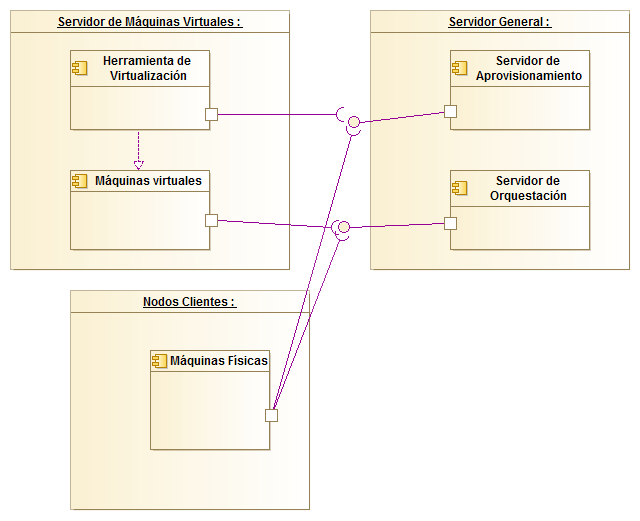
\includegraphics[angle=0]{./figuras/arquitectura_desarrollo.png}}
    \end{figure}

\end{frame}

\begin{frame}{Arquitectura}
    \vspace{0cm} {Diagrama de secuencia}
    \vspace{0.5cm}
    \begin{figure}[ht]
       \centering
       \vspace{-0.50cm}
       \scalebox{0.25}{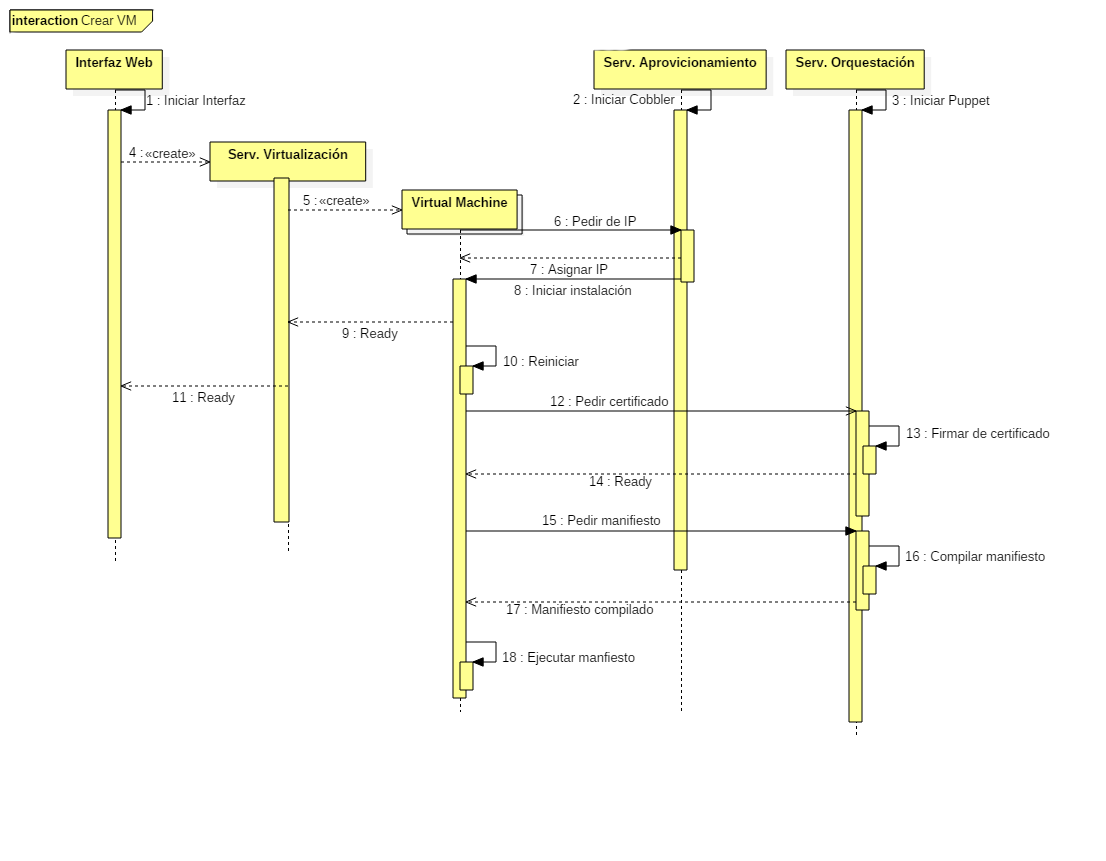
\includegraphics[angle=0]{./figuras/Crear_VM.png}}
    \end{figure}

\end{frame}



%---------------------------------------------------------------------------------------------------------------------------------------------
%                                                                DESARROLLO
%---------------------------------------------------------------------------------------------------------------------------------------------
\section{Desarrollo}
\begin{frame}
    %\vspace{}
    \Huge
    \centering
    \textbf{Desarrollo}

\end{frame}

% -  -  -  -  -  -  -  -  -  -  -  -  -  -
%           VIRTUALIZACION
% -  -  -  -  -  -  -  -  -  -  -  -  -  -

\begin{frame}{Desarrollo - Virtualización}
    \vspace{-1.5cm}
    La herramienta utilizada para virtualizar fue KVM/Qemu.

    KVM utiliza virtualización completa:
    \begin{itemize}
        \item El sistema operativo huésped desconoce que está en un entorno virtual
        \item El hardware se encuentra virtualizado por el sistema operativo anfitrión
        \item La capa de virtualización, el hypervisor, media entre los sistemas huéspedes y el anfitrión
    \end{itemize}

\end{frame}

\begin{frame}{Desarrollo - Virtualización}
    \vspace{0cm} {Esquema de virtualización completa}
    \vspace{0.5cm}
    \begin{figure}[ht]
       \centering
       \vspace{-0.50cm}
       \scalebox{0.60}{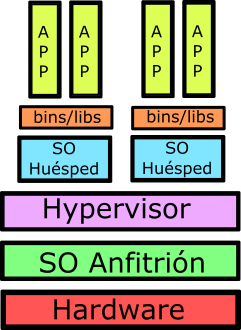
\includegraphics[angle=0]{./figuras/virtualizacion_tipos_3.png}}
    \end{figure}

\end{frame}

\begin{frame}{Desarrollo - Virtualización}
    \vspace{0cm} {Arquitectura de KVM}
    \vspace{0.5cm}
    \begin{figure}[ht]
       %\centering
       \raggedright
       \vspace{-0.50cm} 
       \scalebox{0.25}{\hspace*{4cm}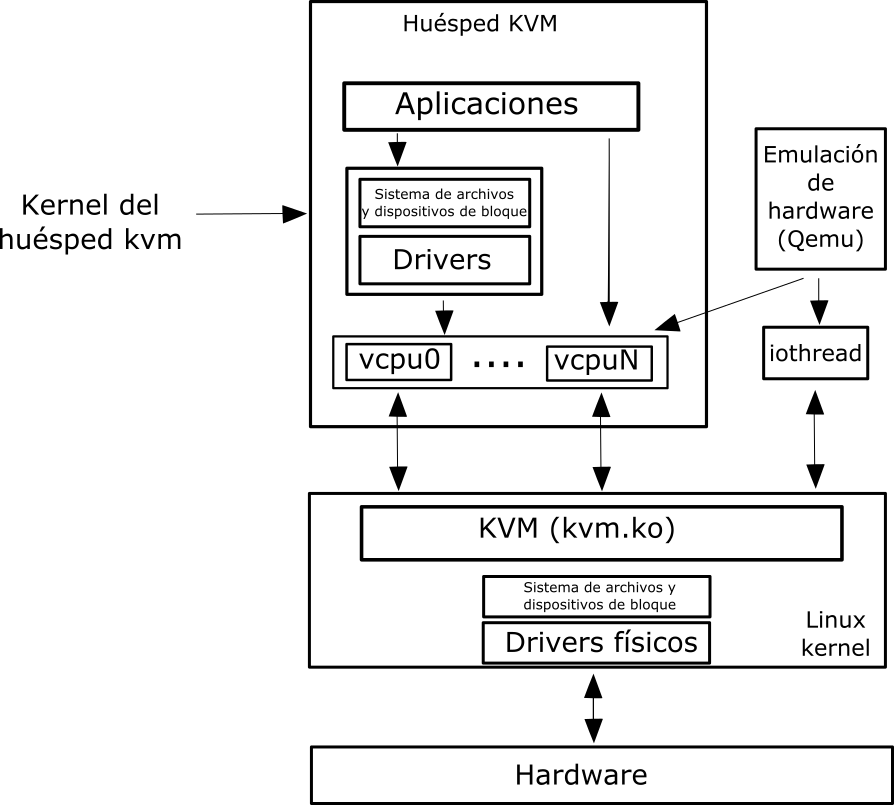
\includegraphics[angle=0]{./figuras/kvm_arquitectura_1.png}}
    \end{figure}

\end{frame}

% -  -  -  -  -  -  -  -  -  -  -  -  -  -
%           APROVISIONAMIENTO
% -  -  -  -  -  -  -  -  -  -  -  -  -  -

\begin{frame}{Desarrollo - Aprovisionamiento}
    \vspace{-1.5cm}
    La herramienta utilizada para el aprovisionamiento fue Cobbler.
    \\
    Utiliza una arquitectura cliente - servidor.
    \begin{itemize}
        \item El servidor debe ejecutarse en un sistema basado en Unix
        \item Centraliza y simplifica el control de servicios incluyendo PXE, DHCP, TFTP y DNS con propósito de realizar instalaciones basadas en red de sistemas operativos
        \item Cobbler utiliza objetos para definir la configuración de aprovisionamiento:
    \end{itemize}
    
\end{frame}

\begin{frame}{Desarrollo - Aprovisionamiento}
    \vspace{0cm} {Modelado de Cobbler}
    \vspace{0.5cm}
    \begin{figure}[ht]
       \centering
       \vspace{-0.50cm}
       \scalebox{0.32}{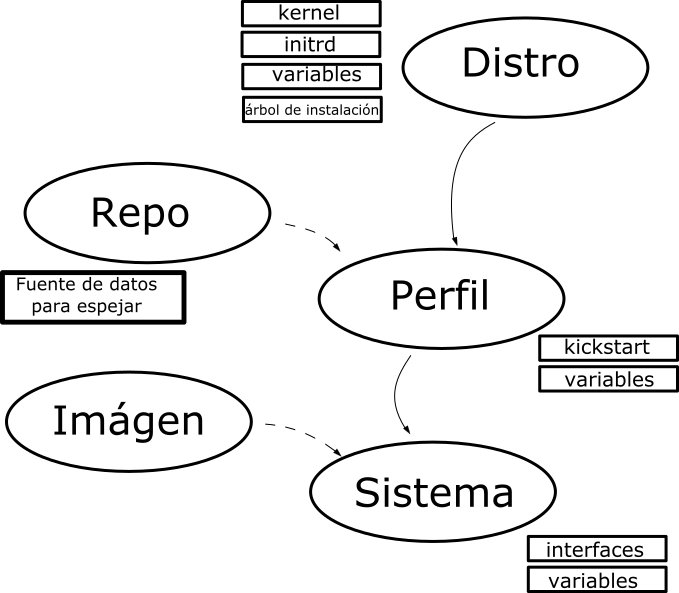
\includegraphics[angle=0]{./figuras/cobbler_modelado.png}}
    \end{figure}
\end{frame}

\begin{frame}{Desarrollo - Aprovisionamiento}
    \vspace{-1.5cm}
    \begin{itemize}
        \item \textbf{Distro}: Distribución que se desea instalar
        \item \textbf{Repo}: Repositorio, sitio centralizado donde se almacena y mantiene información digital
        \item \textbf{Perfil}: Asocia una distribución a opciones especializadas adicionales, como puede ser un archivo de configuración
        \item \textbf{Imágen}: Copia del estado de un sistema computacional, guardado en un archivo o disco
        \item \textbf{Sistema}: Mapea una pieza de hardware (o una máquina virtual) con el perfil asignado a correr en ella
    \end{itemize}

\end{frame}

%\begin{frame}{Desarrollo - Aprovisionamiento}
%    \vspace{0cm} {Distribuciones}
%    \vspace{0cm}
%    \begin{figure}[ht]
%       \centering
%       \scalebox{0.3}{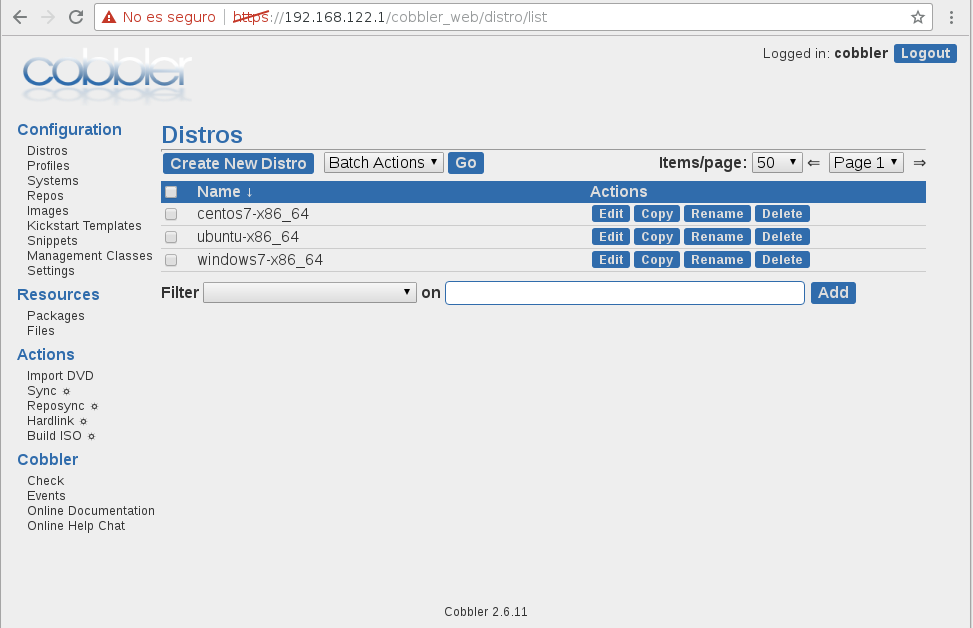
\includegraphics[angle=0]{./figuras/cobbler_web_distros.png}}
%    \end{figure}
%
%\end{frame}
%
%\begin{frame}{Desarrollo - Aprovisionamiento}
%    \vspace{0cm} {Sistemas}
%    \vspace{0cm}
%    \begin{figure}[ht]
%       \centering
%       \scalebox{0.3}{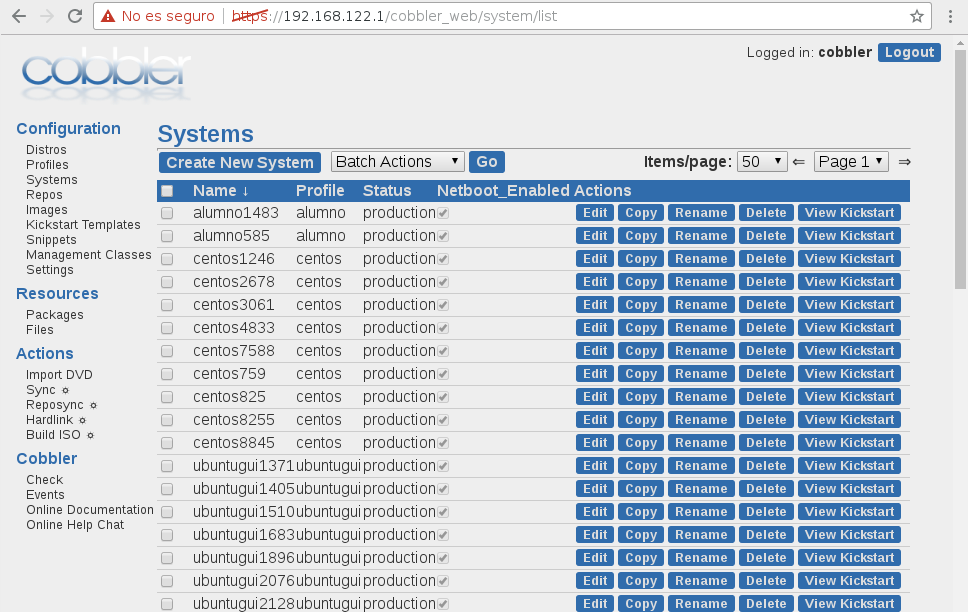
\includegraphics[angle=0]{./figuras/cobbler_web_systems.png}}
%    \end{figure}
%
%\end{frame}
%
%\begin{frame}{Desarrollo - Aprovisionamiento}
%    \vspace{0cm} {Perfiles}
%    \vspace{0cm}
%    \begin{figure}[ht]
%       \centering
%       \scalebox{0.3}{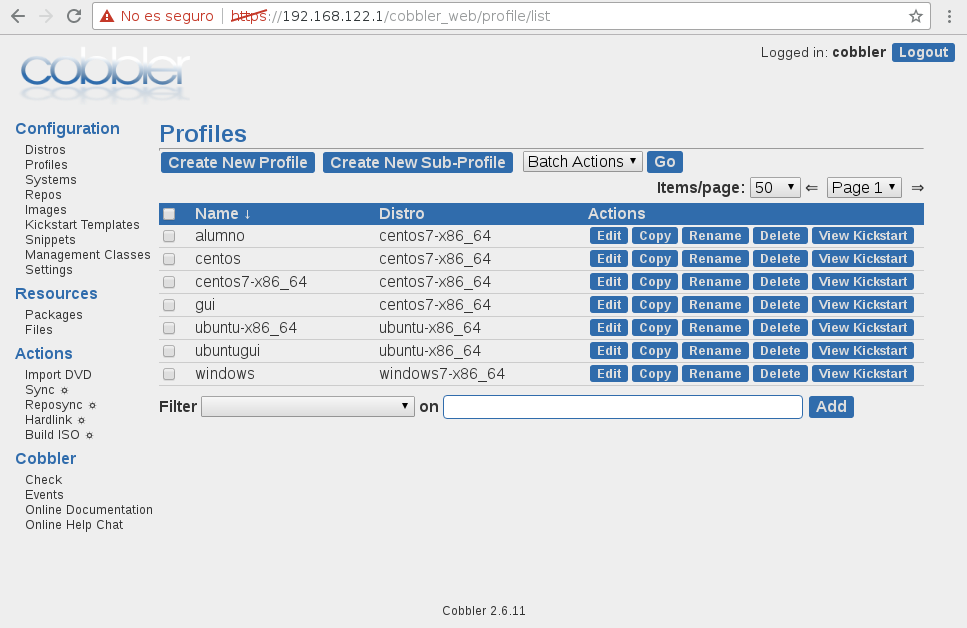
\includegraphics[angle=0]{./figuras/cobbler_web_profile.png}}
%    \end{figure}
%
%\end{frame}
%
%\begin{frame}{Desarrollo - Aprovisionamiento}
%    \vspace{0cm} {Propiedades del perfil}
%    \vspace{0cm}
%    \begin{figure}[ht]
%       \centering
%       \scalebox{0.35}{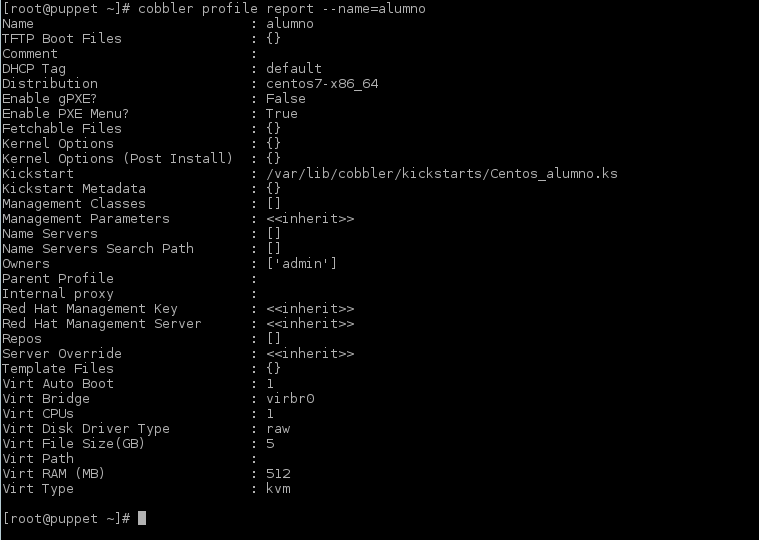
\includegraphics[angle=0]{./figuras/cobbler_terminal_perfil_1.png}}
%    \end{figure}
%
%\end{frame}
%
%\begin{frame}{Desarrollo - Aprovisionamiento}
%    \vspace{0cm} {Propiedades del perfil}
%    \vspace{0cm}
%    \begin{figure}[ht]
%       \centering
%       \scalebox{0.35}{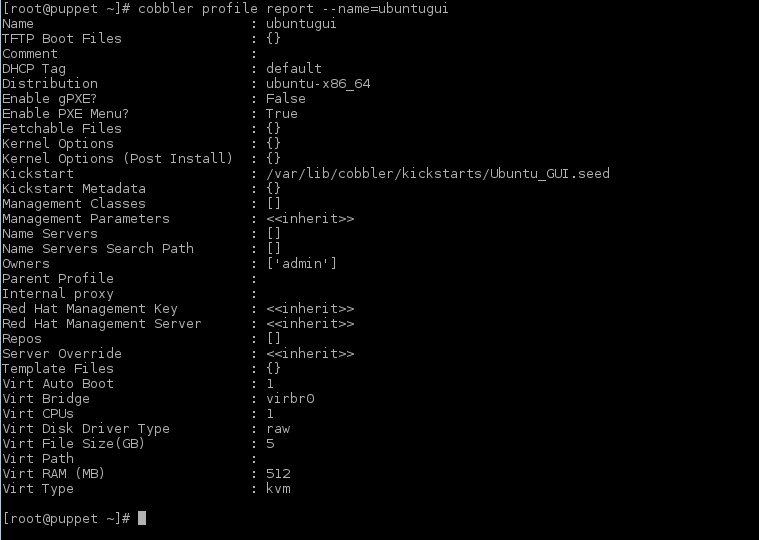
\includegraphics[angle=0]{./figuras/cobbler_terminal_perfil_2.png}}
%    \end{figure}
%
%\end{frame}
%
% -  -  -  -  -  -  -  -  -  -  -  -  -  -
%           ORQUESTACION
% -  -  -  -  -  -  -  -  -  -  -  -  -  -

\begin{frame}{Desarrollo - Orquestación}
    \vspace{-1.5cm}
    La herramienta utilizada para orquestar fue Puppet.
    \\
    Utiliza una arquitectura cliente - servidor.  
    \begin{itemize}
        \item El servidor (nodo maestro) debe ejecutarse en un sistema basado en Unix
        \item Los clientes (agentes) soportan múltiples plataformas
        \item Posee su propio DSL (Domain Specific Language)
        \item El usuario describe los recursos del sistema y sus estados utilizando un lenguaje declarativo  
        \item El nodo maestro provee una interfaz HTTPS con varios extremos disponibles
        \item Cuando se pide o envía cualquier dato al servidor, el agente hace un pedido HTTPS o a uno de esos extremos
    \end{itemize}

\end{frame}


\begin{frame}{Desarrollo - Orquestación}
    \vspace{0cm} {Ciclo de Puppet}
    \vspace{0cm}
        \begin{figure}[ht]
           \centering
           \scalebox{0.38}{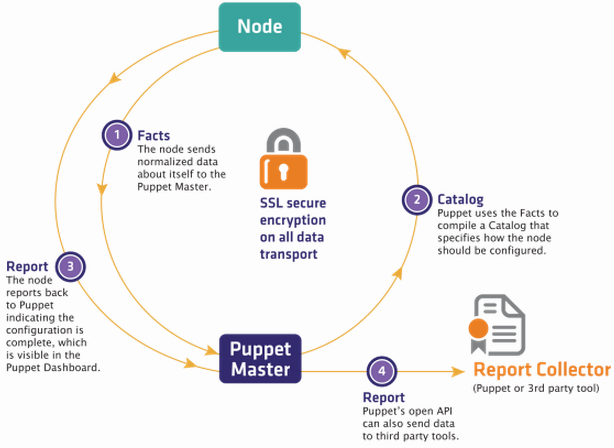
\includegraphics[angle=0]{./figuras/puppet_funcionamiento.png}}
        \end{figure}

\end{frame}

%\begin{frame}{Desarrollo - Orquestación}
%    \vspace{0cm} {Nodos administrados}
%    \vspace{0cm}
%    \begin{figure}[ht]
%       \centering
%       \scalebox{0.6}{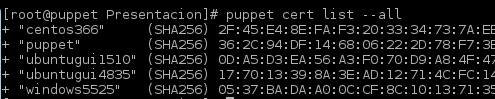
\includegraphics[angle=0]{./figuras/puppet_nodos.png}}
%    \end{figure}
%
%\end{frame}

\begin{frame}{Desarrollo - Orquestación}
    \vspace{0cm} {Estructura de los módulos de Puppet}
    \vspace{0cm}
    \begin{figure}[ht]
       \centering
       \scalebox{0.3}{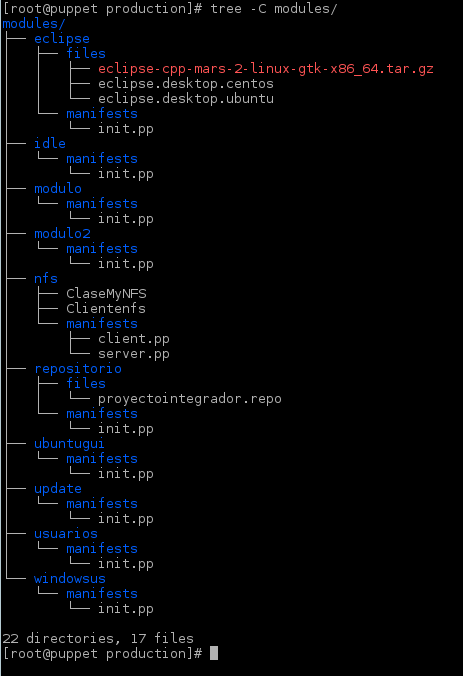
\includegraphics[angle=0]{./figuras/puppet_modulos.png}}
    \end{figure}

\end{frame}

% -  -  -  -  -  -  -  -  -  -  -  -  -  -
%           INTERFAZ WEB
% -  -  -  -  -  -  -  -  -  -  -  -  -  -

\begin{frame}{Desarrollo - Interfaz Web}
    \vspace{-1.5cm}
    La herramienta utilizada para crear la interfaz web fue Python Bottle.
    Utiliza una arquitectura cliente - servidor.
    \begin{itemize}
        \item Es un WSGI (Web Server Gateway Interface) rápido, sencillo y ligero
        \item Distribuído como un módulo único
        \item Su única dependencia es la Librería Estándar de Python
        \item Puede ejecutarse como un servidor web autónomo
        \item Plugins para bases de datos populares
    \end{itemize}
    
\end{frame}

\begin{frame}{Desarrollo - Interfaz Web}
    \vspace{0cm} {Crear múltiples máquinas virtuales}
    \vspace{0cm}
    \begin{figure}[ht]
       \centering
       \scalebox{0.3}{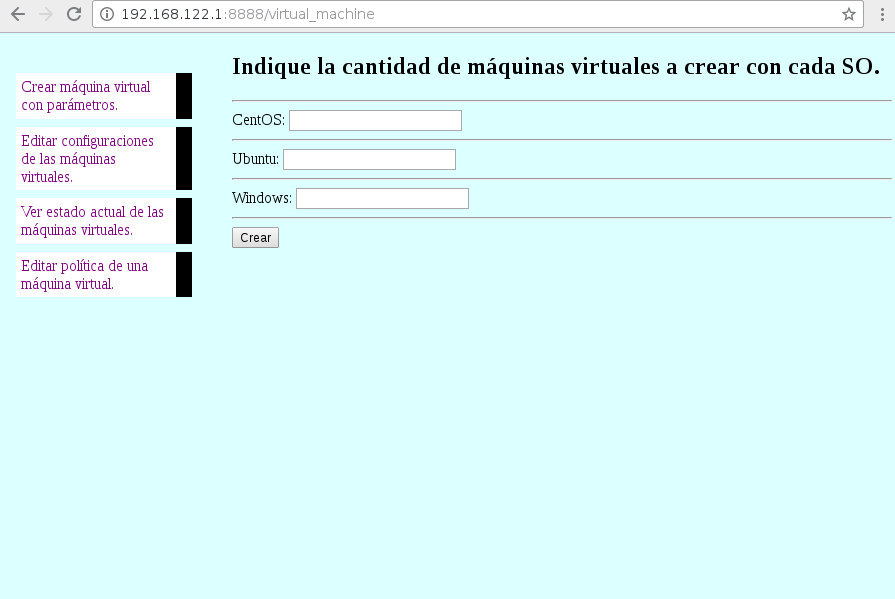
\includegraphics[angle=0]{./figuras/interfaz_web_1.png}}
    \end{figure}

\end{frame}

\begin{frame}{Desarrollo - Interfaz Web}
    \vspace{0cm} {Aplicar políticas por sistema operativo}
    \vspace{0cm}
    \begin{figure}[ht]
       \centering
       \scalebox{0.3}{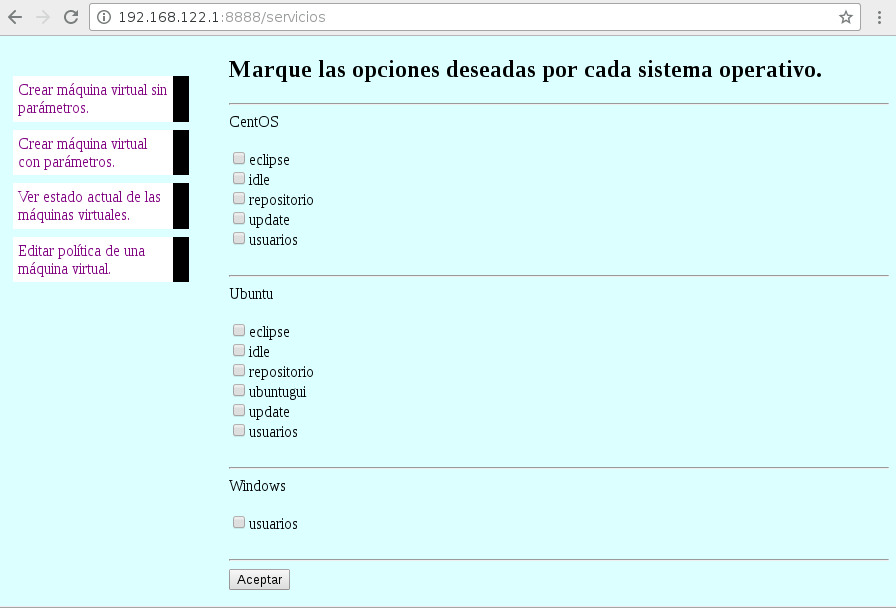
\includegraphics[angle=0]{./figuras/interfaz_web_2.png}}
    \end{figure}

\end{frame}

\begin{frame}{Desarrollo - Interfaz Web}
    \vspace{0cm} {Aplicar políticas por máquina específica}
    \vspace{0cm}
    \begin{figure}[ht]
       \centering
       \scalebox{0.3}{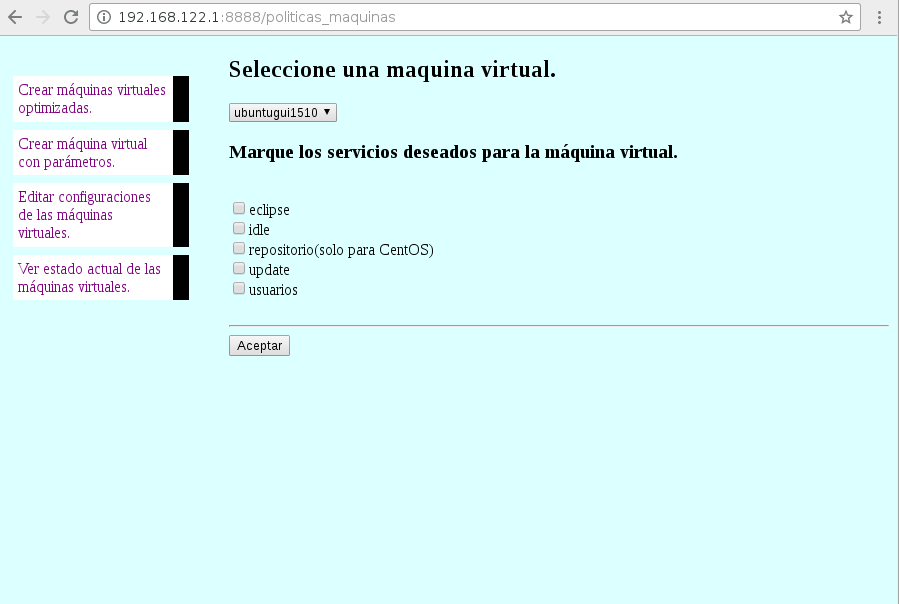
\includegraphics[angle=0]{./figuras/interfaz_web_3.png}}
    \end{figure}

\end{frame}

\begin{frame}{Desarrollo - Interfaz Web}
    \vspace{0cm} {Ver estado de las máquinas}
    \vspace{0cm}
    \begin{figure}[ht]
       \centering
       \scalebox{0.3}{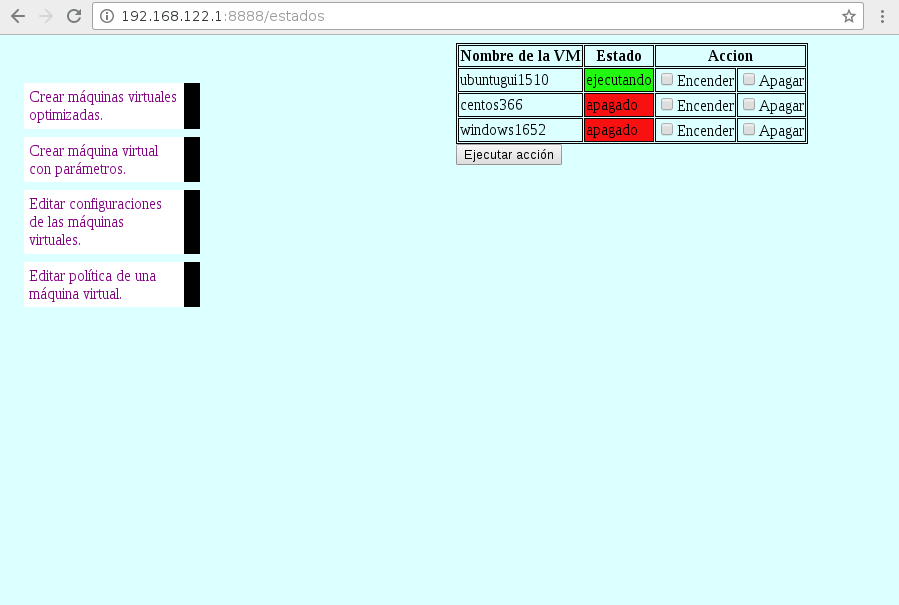
\includegraphics[angle=0]{./figuras/interfaz_web_4.png}}
    \end{figure}

\end{frame}


%---------------------------------------------------------------------------------------------------------------------------------------------
%                                                         VIDEO DEMOSTRACIÓN
%---------------------------------------------------------------------------------------------------------------------------------------------
\section{Video demostración}
\begin{frame}
    %\vspace{}
    \Huge
    \centering
    \textbf{Video demostración}

\end{frame}

\begin{frame}{Video demostración}
    \vspace{-1.5cm}
    \begin{itemize}
        \item Creación de las máquinas virtuales
        \item Aprovisionamiento de las máquinas con el sistema operativo deseado
        \item Orquestar las políticas definidas para una máquina o un conjunto de máquinas
    \end{itemize}

\end{frame}


%---------------------------------------------------------------------------------------------------------------------------------------------
%                                                               CONCLUSIONES
%---------------------------------------------------------------------------------------------------------------------------------------------
\section{Conclusiones}
\begin{frame}
    %\vspace{}
    \Huge
    \centering
    \textbf{Conclusiones}

\end{frame}

\begin{frame}{Conclusiones}
    \vspace{0cm}
    \begin{itemize}
        \item Elección del entorno realizado utilizando factores de decisión ponderados
        \item Solución modularizada
        \item Permite la escalabilidad necesaria
        \item Soluciones de código abierto no siempre permiten estar en la "cresta de la ola"
        \item El sistema final cumple con los requerimientos
    \end{itemize}

    % El análisis formal del problema para la obtención de los requerimientos y los riesgos del proyecto, es algo que también debe destacarse. Esta es una fase imprescindible para poder llevar a cabo las estimaciones pertinentes a los tiempos de desarrollo e investigación de cualquier proyecto. En muchas ocasiones se cuenta con diferentes herramientas para llevar a cabo una misma tarea. El análisis de cada una de ellas y su elección, utilizando factores de decisión ponderados, es fundamental para el trabajo como ingeniero. De aquí también se puede hacer notar que la utilización de soluciones de código abierto no siempre permiten estar en la "cresta de la ola" tecnológica y muchas veces es necesario contar con software privativo para obtener la máxima producción.

    % El resultado final es positivo. El sistema final cumple con los requerimientos, es capaz de generar una gran cantidad de máquinas virtuales completamente equipadas y preparadas para desempeñar diferentes funciones, ya sean académicas o en entornos laborales, formando parte de una red nat con la cual cada máquina puede comunicarse con las demás máquinas de la red y tener acceso a internet.

\end{frame}


%---------------------------------------------------------------------------------------------------------------------------------------------
%                                                        TRABAJOS FUTUROS
%---------------------------------------------------------------------------------------------------------------------------------------------
\section{Trabajos Futuros}
\begin{frame}
    %\vspace{}
    \Huge
    \centering
    \textbf{Trabajos Futuros}

\end{frame}

\begin{frame}{Trabajos Futuros}
    \vspace{0cm}
    \begin{itemize}
        \item Protección: 
        \begin{itemize}
            \item  Modificar el sistema para que funcione con firewall y SELinux
            \item  Incluir autenticación por usuario en la interfaz web
            \item  Incluir un log de cambios al sistema que permita saber quién y qué cambio realizó
        \end{itemize}
        \item Migración: Poder realizar el traslado de hosts virtuales entre las diferentes máquinas físicas
        
    \end{itemize}

\end{frame}

%---------------------------------------------------------------------------------------------------------------------------------------------
%                                                                Q & A
%---------------------------------------------------------------------------------------------------------------------------------------------
\section{Preguntas}
\begin{frame}
    %\vspace{}
    \Huge
    \centering
    \textbf{Preguntas}

\end{frame}
%---------------------------------------------------------------------------------------------------------------------------------------------
%                                                           AGRADECIMIENTOS
%---------------------------------------------------------------------------------------------------------------------------------------------
\section{Muchas Gracias!}
\begin{frame}
    %\vspace{}
    \Huge
    \centering
    \textbf{Muchas Gracias!}

\end{frame}

%---------------------------------------------------------------------------------------------------------------------------------------------
%                                                                 END
%---------------------------------------------------------------------------------------------------------------------------------------------
\end{document}

              